\documentclass[12pt]{article}
\usepackage{amsmath}
\usepackage{amssymb}
\usepackage{graphicx}
\usepackage{color}
\usepackage{float}
\begin{document}	
	\title{Chromatin architecture post UVC irradiation}
\maketitle
\section{Introduction}
    Maintaining the integrity of cellular genome and epigenome is one of the key elements allowing correct gene regulatory function. The constant exposure of the cellular genome to various sources of DNA damages imposes threat to the integrity of both the genetic and epigenetic information. Complete or partial failure to restore the damaged genetic information might lead to apoptosis and development of cancer [REF].
    
    Although several genetic repair pathways are well known [REFs], restoration of epigenetic information has only gained attention recently [REFs]. Disruption of the chromatin architecture, involving chromatin de-compaction and cross-link break, have been recently shown to induce cancer [REF]. It is therefore fundamental to understand how the cell restores chromatin architecture required for normal gene regulation after damages.
    
	Our current understanding of the repair process is based on the Access-Repair-Restore model suggested by [REF]. Accordingly, following the detection of DNA lesion [REF] repair protein are recruited to DNA damage sites. To facilitate efficient access to DNA histones are removed, cross-links are broken and the chromatin in the micro-environment is generally de-compacted. Upon repair, repair proteins leave the damage region promoting the initiation of deposition of old and newly synthesized histones back into the chromatin and subsequently promoting chromatin compaction.
    
    Recently, experiments following the dynamics of tagged histones and DNA post UV-C, show a great imbalance between histone and DNA signal loss. This imbalance implies that chromatin de-compaction and expansion around the damage zone operates in parallel to exclusion of histones. %explain about sliding of histones as a potential mechanism 
    Many structural changes are involved in the process of repair [REF].  Induction of UV-C light on chromatin, in the exposure time 0-120 promotes nucleotide fusion and activates the Nucleotide Excision Repair mechanism [REF].
    
	To estimate the nucleosome reorganization following DNA damages, we have
	constructed a mathematical model, where redistribution can be due either to chromatin de-compaction or nucleosome sliding along the chromatin or both of them. We have used the model to assess the relative contribution of these two processes to the total DNA and nucleosome signal loss from a region of interest (ROI), a quantity which is inaccessible experimentally.
	
	The model (presented in Material and methods) follows the DNA, $D(u)$,
	and nucleosome, $H(u)$, fraction of signal loss from the ROI as a function of
	the UV dose, $u$. We have used the measured H3.3 and DNA signal loss to
	calibrate parameters of nucleosome and DNA models respectively.
	
	We use the result of the analytical model to calibrate an \textit{in-silico} simulation of chromatin. We perform simulations in line with the experimental procedure to explore and compare functional healthy chromatin before UV damage to that post repair. % missing the results of the smimulations 
		
 \section{Material and Methods} 
	
	We present here a model for nucleosomes and DNA re-organization following
	UV damages. The cascade of events leading to tagged DNA and nucleosomes'
	redistribution, results in signal extrusion from a region of interest (ROI) up
	to a maximal loss, measured 15 minutes post UV-C.
	
 \subsection{The experimental procedure}
	Following the experimental protocol in \cite{adam2015imaging}, a two-dimensional initial damage region (DR), induced by the UV-C laser, is centered around the laser's focal point (Figure \ref{fig:ExperimentalProcedure} box A). Post UV-C the damaged region-- visualized by GFP-XPC, GFP-NER and tagged nucleosomes-- expands radially outward and reach its maximal area after 15 minutes (Figure \ref{fig:ExperimentalProcedure} box B). At the end of expansion, the region is defined as the ROI, in which DNA and nucleosome signals are measured and compared to signals measured in the ROI just prior to UV irradiation. The fraction of signal loss is calculated as the difference between the two measurements relative to time 0.
	
	\subsection{Modeling nucleosomes and DNA redistribution following UV damages}
		\begin{figure}[H]
			\centering
			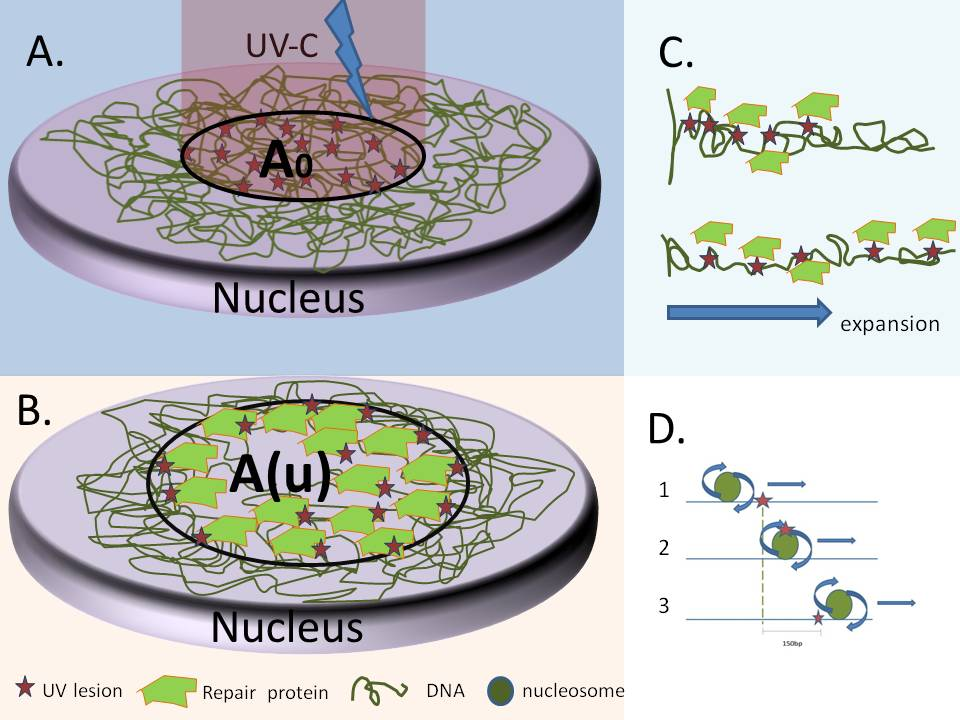
\includegraphics[width=0.7\linewidth, height=0.4\textheight]{ExperimentalProcedure}
			\caption{\small{\textbf{Expansion of the ROI post UV-C as a result of chromatin de-compaction and nucleosome sliding.} \textbf{A.} illumination of UV-C (red cylinder) in the initial damage region (DR) of area $A_0$ create uniformly distributed UV lesions (red stars) shows repair proteins (green polygons) de-compact the chromatin to access DNA damages. Additionally, to facilitate efficient repair, DNA is exposed by sliding nucleosomes. Chromatin de-compaction and nucleosome sliding expand the DR up to a maximal area $A(u)$ (the ROI), reached 15 minutes post UV-C irradiation \textbf{C.} expansion of the DR due to DNA de-compaction by chromatin remodlers and repair proteins results in equal proportion of DNA and nucleosome signal extrusion from the ROI \textbf{D.} nucleosome sliding allows additional loss of nucleosome signal. Three time points on a 1D representation shows the principle of nucleosome signal loss with no DNA signal loss from the ROI. Nucleosomes (green circle) sliding over a UV lesion (red star) displaces the lesion spatially by a distance equivalent to length of DNA wrapped on a histone ($\approx150 bp$) }. As nucleosome slide, tagged repair protein will bind to newly exposed damage points, thus expanding the DR while retaining all UV lesions in it.}
			\label{fig:ExperimentalProcedure}
		\end{figure}
		
	Experimental data shows a higher proportion of nucleosome signal loss than DNA for all UV dose (Figure \ref{fig:histoneAndDnaVsUvDoseModelFit}). To explain this observation we assume that the loss of DNA and nucleosome signals post UV-C is due to two mechanisms: the first is chromatin expansion, and the second is nucleosomes sliding along the chromatin. 
	
	For chromatin expansion, recruitment of repair and chromatin remodeling factors to bind to damaged DNA causes chromatin de-compaction and cross-links break to facilitate efficient repair \cite{gaillard2003chromatin,luijsterburg2012ddb2,deem2012epigenetic}. Accumulation of repair factors in the DR will generate a pushing force on surrounding chromatin in a radial outward direction \cite{dinant2007activation}. As a result, DNA and nucleosome outside the DR will be extruded from the ROI in equal proportions (Figure \ref{fig:ExperimentalProcedure} box A-C).
	
	An additional proportion of nucleosome signal loss is caused by the mechanism of nucleosome sliding. This mechanism allows nucleosome signal loss with no additional DNA signal loss. Repair proteins slide nucleosomes wrapped by damaged DNA away from high concentration of DNA damages to expose damaged DNA \cite{gaillard2003chromatin}. As a result the chromatin in the DR will loosen and remodeling and repair proteins will bind to the exposed damaged sites. This further contribute to the pushing of undamaged DNA outside the DR while retaining damaged DNA within it (Figure \ref{fig:ExperimentalProcedure} box D).  

    In-line with the description above, we construct a model representing
	signal loss 15 minutes post UV-C as a function of the UV dose. We do not take into account the
	mechanism of signal loss in time and only present equations representing the maximal loss of signal 15 minutes post UV-C.
	

	\subsection{Dynamics of DNA and nucleosome loss from the DR}
	The DR and the ROI are considered to be two-dimensional concentric circular regions, characterized by an area $A_0$ and $A(u)$, respectively (Figure \ref{fig:ExperimentalProcedure} box A,B). We assume an initial uniform distribution of DNA in the DR and its vicinity, such that the amount of DNA in $A(u)$ is $c_dA(u)$, with $c_d$ in units of $bp/\mu m^2$. 
	
	We restrict DNA damages to be inflicted only in $A_0$ immediately after UV induction. We set $T(u)$ to represent the amount of damaged DNA left in $A(u)$ 15 minutes post UV-C, while the undamaged DNA is assumed to be extruded. Therefore, the fraction of DNA signal loss, $D(u)$, is calculated as the ratio of extruded DNA to the total amount of DNA in the ROI, $c_dA(u)$. 
	\begin{equation}\label{eq:DNALossFraction}
	D(u) = \frac{c_dA(u)- T(u)}{c_dA(u)}
	\end{equation}
	
	We set the number of nucleosomes in a $A(u)$ to be $c_nA(u)$, with $c_n$ a constant in units of $nucleosomes/\mu m^2$. The total fraction of nucleosome extruded from the ROI, $H(u)$, is calculated as the sum of nucleosomes extruded along with undamaged DNA and the ones sliding out.
	\begin{equation}\label{eq:nucleosomeLossFraction}
	H(u) = D(u) + \frac{N_S(u)}{c_nA(u)}	
	\end{equation}
	
	In order to evaluate the fractions in \eqref{eq:DNALossFraction} and \eqref{eq:nucleosomeLossFraction}, we shall first formulate a model for the damaged DNA in the DR, $T(u)$ and derive $A(u)$ and $N_S(u)$ based on it.
	
	\subsection{DNA damages in the DR as a function of the UV dose}\label{subsection:AccumulationOfDNADamagesInTheDR}
	 We assume that the number of DNA damages in $A_0$ follows a homogeneous Poisson point process. As the UV exposure time increases, we assume that the mean number of damages per $\mu m^2$ increases as $k_tu$, with $k_t$ in units of $bp/(msec\times \mu m^2)$. Because no two damages can occur on the same position on the DNA, the rate of accumulation of DNA damages with UV dose can be written as
	\begin{equation}\label{eq:DNADamageRate}
	\frac{dT(u)}{du} = k_tu(c_dA_0 - T(u))
	\end{equation}	
	 Using the initial condition $T(0) = 0$, the solution to equation \eqref{eq:DNADamageRate} is
	\begin{equation}\label{eq:DNADamageDR}
		T(u) = c_dA_0(1-\exp(-k_tu^2))
	\end{equation}
	
	\subsection{The number of nucleosomes sliding out of the DR}
	We now turn to construct a model for the number of nucleosomes $N_S(u)$
	sliding out of the DR and subsequently out of the ROI as a function of the UV dose. Although the exact mechanism by which nucleosome are lost is not known, 
	we propose that the rate of nucleosomes sliding out is proportional to the fraction of nucleosomes affected by increase of UV dose in $A_0$. In the first-order approximation, the dynamics of nucleosomes sliding is given by
	\begin{equation}\label{eq:nucleosomeSlideRate}
	\frac{dN_S(u)}{du} = k_s\left(c_nA_0-N_S(u))\right)\frac{dT(u)}{du}	 
	\end{equation}
	with $k_s$ a constant of units $1/bp$. Using the initial condition $N_S(0)=0$, the solution to equation \eqref{eq:nucleosomeSlideRate} is 
	\begin{equation}\label{eq:nucleosomeSlideDR}
	N_S(u)= c_nA_0\left(1-\exp(-k_sT(u))\right)
	\end{equation}
	with $T(u)$ defined in equation \eqref{eq:DNADamageDR}.
   \subsection{The ROI expansion}
	Next, we model the dynamics of the ROI area $A(u)$ with increasing UV
	dose. For this end, we consider the ROI area to expand as a result of the de-compaction of the damaged DNA, and by the effect of nucleosome sliding. 			
	\begin{equation}\label{eq:RoiAreaGrowthRate}
	\frac{dA(u)}{du}=k_a\frac{dN_S(u)}{du}+k_b\frac{dT(u)}{du}
	\end{equation}
	where $k_a$ is a constant of units $\mu m^2/ nucleosomes$ and $k_b$ of units $\mu m^2/ bp$. Using the initial condition $A(0) = A_0$, the solution to equation \eqref{eq:RoiAreaGrowthRate} is
	\begin{equation}\label{eq:RoiArea}
	A(u) = A_0+ k_ac_nA_0\left(1-\exp(-k_sT(u))\right)+k_bT(u)
	\end{equation}
	 with $A_0$ representing the size of a DR even in the absence of UV irradiation.
	 
	 \subsection{Final expression for DNA $D(u)$ and nucleosome $H(u)$ signal loss}
	We can now substitute the functions \eqref{eq:DNADamageDR}, \eqref{eq:nucleosomeSlideDR}, \eqref{eq:RoiArea} into the equations \eqref{eq:DNALossFraction} and \eqref{eq:nucleosomeLossFraction} to get the expressions for $D(u)$ and $H(u)$. We present the result in terms of $T(u)$
	\begin{equation}\label{eq:DNALoss}
	D(u) = 1-\frac{1}{1+ k_ac_n\left(1-\exp(-k_sT(u))\right)+k_bT(u)/A_0} 
	\end{equation}
	\begin{equation}\label{eq:nucleosomeLoss}
		H(u) = 1- \frac{\exp(-k_sT(u))}{1+ k_ac_n\left(1-\exp(-k_sT(u))\right)+k_bT(u)/A_0}
	\end{equation}
		\subsection{Parameter fit for $D(u)$ and $H(u)$}\label{subsection:parameterFit}
	     We simultaneously fit equations \eqref{eq:DNALoss}  and \eqref{eq:nucleosomeLoss} to the H3.3 and DNA loss data, with the goal of maximizing the $R^2$ of both equations. Excluding the measurement at 5 msec, and using classical fitting procedure, we find
		\begin{equation*}
		k_t = 8\times 10^{-4}, \quad k_sc_dA_0 = 0.31,\quad k_ac_n = 0.29, \quad k_bc_d = 0.24
		\end{equation*}
		with $R^2 = 0.94$ and $R^2 = 0.955$ for DNA and nucleosome loss fit respectively.
		
			

\subsection{Relative contribution of opening and sliding to DNA
	and nucleosome signal loss}

Using the calibrated model in equation equations \eqref{eq:DNALoss} and \eqref{eq:nucleosomeLoss}, we now calculate the
relative contribution of chromatin opening and nucleosome sliding to the
total loss of DNA and nucleosome signals. The sliding contribution refers to all loss
caused by either directly sliding nucleosome out of the DR or as the effect
nucleosome sliding has on pushing chromatin out of the DR. Chromatin opening contribution refers to all signal loss caused by chromatin remodeling.

We start by partitioning equation \eqref{eq:RoiArea}, describing the ROI into the two sub-mechanisms contributing to its expansion 
\begin{equation*}
A(u) = A_P(u) +A_S(u)
\end{equation*}
with $A_P(u)=A_0+k_bT(u)$, the area attributed to chromatin opening, and $A_S(u)=k_aN_S(u)$ to nucleosome sliding. 

The fraction of DNA signal loss attributed to chromatin opening is calculated similarly to equation \eqref{eq:DNALossFraction} as 
\begin{equation*}
D_P(u)=\frac{c_dA_P(u)-c_dA_0}{c_dA(u)}
\end{equation*}
The relative contribution of chromatin opening to the total DNA signal loss is therefore,
\begin{equation}\label{eq:relativeOpeningDNA}
\frac{D_P(u)}{D(u)}=\frac{A_P(u)/A_0-1}{A(u)/A_0-1}
\end{equation}	
The relative contribution of nucleosome sliding to the total DNA signal loss is
\begin{equation}\label{eq:relativeSlidingDNA}
\frac{D_S(u)}{D(u)}=1-\frac{D_P(u)}{D(u)}
\end{equation}

The relative contribution of chromatin opening and nucleosome
sliding to the total nucleosome signal loss is given respectively by
\begin{eqnarray}
\frac{H_P(u)}{H(u)} &=& \frac{D_P(u)}{H(u)}\label{eq:relativeOpeningNucleosomes}\\
\frac{H_S(u)}{H(u)} &=&1-\frac{H_P(u)}{H(u)} \label{eq:relativeSlidingNucleosomes}
\end{eqnarray}
where here we have used the fact that $H_P(u) = D_P(u)$, i.e fraction of nucleosomes extruded from the ROI along with undamaged DNA. Graphs of



\section{The simulation framework}
	To examine the similarity between the chromatin conformation before UV-C and after repair, we follow \textit{in-silico} the dynamics of DNA and nucleosome signal loss from a circular region of interest (ROI).
	
	The UV beam is consider to affect each horizontal slice of the nucleus in a similar manner \cite{adam2015imaging}. Therefore, we perform two-dimensional simulations in spherical domain with reflecting boundaries. Our simulation capture the UV damage micro-environment and not the entire nucleus. Simulations are performed for UV-C dosage $u$ ranging from 0 to 120 msec exposure.  

	
	\subsection{The polymer model}
	We use a randomly cross-linked Rouse chain of $N$ monomers connected by harmonic springs \cite{doi1988theory} to represent a coarse-grained model of the chromatin. Springs connecting adjacent monomers in the linear chain are allowed to contract to a minimal length $L_0>0$. Cross-links are represented by harmonic springs connecting a subset of $M\leq N$ non nearest-neighbor (NN), who allowed to contract to a minimal length $L_C>0$.  
	
	The measure of cross-linking is given by the fraction $0\leq \alpha\leq 1$ of non-NN monomers connected out of the total possible connectivity. For a polymer of $N$ monomers, the number of connectors associated with $\alpha$ is thus 
	$\lfloor\alpha(N-2)(N-1)/2\rfloor$.
		
	The position $R_n$ of the $n^{th}$ monomer of the chain is represented by the equation 
	\begin{equation}
	\frac{\partial R_n}{\partial t}(t) = \sum_m H_{nm}\left(-\frac{\partial U_0}{\partial R_m(t)}+g_m(t)\right) -\sum_m \hat{H}_{nm}\frac{\partial U_{L_c}}{\partial R_m (t)}
	\end{equation}
	where $H_{nm}=\frac{\delta_{nm}}{\zeta}$ is the mobility tensor of the linear chain, and 	
	\begin{equation}
	\hat{H}_{nm}= \begin{cases}
	\frac{1}{\zeta},\qquad 
	\text{if monomer \textit{n} and \textit{m} are connected ($n\neq m$)}\\
	0,\qquad \text{else}
	\end{cases}
	\end{equation}
	is the mobility tensor for the cross-linked monomers. 
	The terms $g_m$ are white noise with zero mean and std equals $2\zeta k_BT$, with $\zeta$ the friction constant, $k_B$ is the Boltzmann constant, and $T$ the temperature.  
	
	The spring potential energy with minimal length $L$ is defined by  
	\begin{equation}
	U_L=\frac{3k_BT}{2b^2}\sum_{n=1}^N (||R_{n}-R_{n+1}||^2-L)^2
	\end{equation}
    with $b>L$ the std of spring length. 
    		
	For each realization of the polymer, cross-links are added between pairs of monomers chosen uniformly at random corresponding to the values of $\alpha$. The dynamics of the cross-linked polymer is then simulated up to its relaxation time, determined by be the slowest mode of the linear chain \cite{doi1988theory}.

	\subsection{UV irradiation}
	At the end of relaxation steps an instantaneous UV beam is shot with its focal point placed at the polymer's center-of-mass (CM). Small fluctuations of monomers are not of interest at the scale of our simulation, therefore the diffusion force acting on the polymer is stopped at this point. Damages caused by UV are restricted to be contained within a fixed two-dimensional circular region of area $A_0$ centered at laser's focal point. [EXPLAIN ABOUT THE DAMAGES]
	
	Damages to DNA are represented by monomers labeled as damaged. For each UV dose $u$, damages caused by UV are uniformly distributed between  monomers in $A_0$ at the time of beam shot. With increase of UV dose, we increase the probability of damages linearly as $k_tu$, with $k_t$ in units of $bp/msec$. 
	
	\subsubsection{The repair stage}	
	To simulate the affect of repair proteins crowding at sites of DNA damage, a circular exclusion region is centered at each damaged monomer. An elastic pushing force originating from the damaged monomer and having affect radius $r_p$ is applied on any monomers entering the exclusion region. In addition, all cross-links from and to damaged monomers are removed to simulate chromatin de-compaction caused by the activity of chromatin remodlers and repair proteins \cite{gaillard2003chromatin}. 
	
	The polymer will evolve into a new steady spatial configuration which represents the chromatin 15 minutes post UV-C. At which point, the region of interest (ROI) is defined as the circle containing 90\% of the damaged monomers and centered at their CM. The ROI remains a fixed region used to track the number of damaged and undamaged monomers within it. Measurements are done off-line, such that the ROI's position is retrospectively updated to be centered at the CM of the monomers tagged damaged.
	
	\begin{figure}[H]
	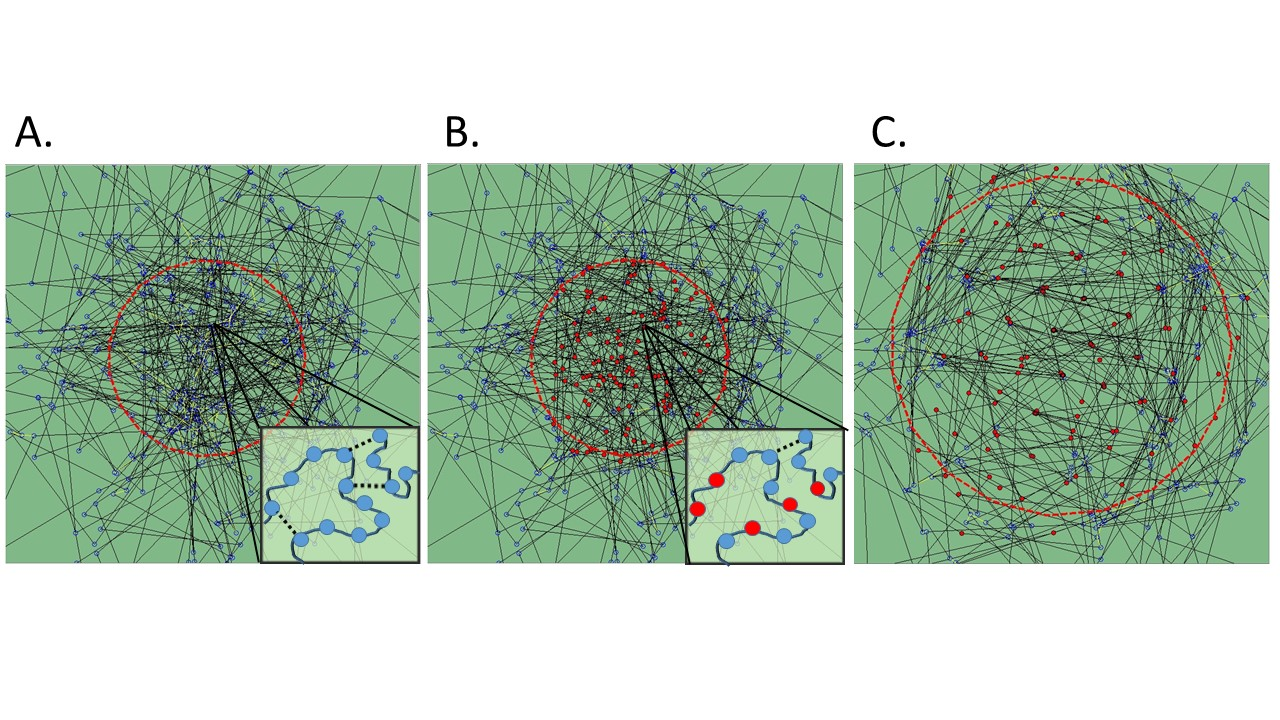
\includegraphics[width=0.9\linewidth, height=0.35\textheight]{threeStagesOfSimulation}
	\caption{\textbf{Stages in the Simulation of chromatin spatial organization post UV-C irradiation}. \textbf{A.} a Rouse chain of 500 monomers (circles) connected by harmonic spring (black lines) with a minimal length L0 is crossed-linked by harmonic springs (dashed lines in box) is simulated up to relaxation time, at which point a UV-C beam is vertically shot through a circular damage region (red dashed circle) around the polymer’s center-of-mass. \textbf{B.}  damaged monomers (red circles) are set to be distributed uniformly for each UV dose. Following UV-C irradiation, cross-links (dashed lines in box) to and from damaged monomers are removed. \textbf{C.} crowding of repair proteins is simulated by regions of exclusion centered around each damaged monomer. An elastic pushing force is applied to surrounding monomers with a maximal affect radius of rp. As a result, the damage region expands until reaching its maximal size 15 minutes post UV-C. The Region of Interest (ROI) is then determined as the circles containing 90\% of the damaged monomers (dashed red circle).}
	\label{fig:threeStagesOfSimulation}
	\end{figure}
	
	\subsection{Post repair stage}
	Damaged monomers are repaired with time dependent probability. The exclusion region is removed once a monomer is repaired and cross-links are allowd to be formed to other repaired or non-damaged monomers.  Cross-links are reintroduced by linking any two monomers located within an encounter distance of $\epsilon$ from one another. Cross-links post repair are allowed to be added up to the initial cross-linking percentage $\alpha$.
	
	\subsection{Measuring structural similarity}
	A measure of similarity between the polymer spatial organization before UV and post repair is based on the comparison of their encounter probability matrices. Encounter probability matrix is obtained by dividing each cell $i,j$ in the encounter frequency matrix by the total number of encounter of monomer $i$ and $j$. The polymer's encounter matrix just prior the onset of UV-irradiation is compared to that at end simulation time. The similarity values is given by the mean square error between matrices. 
	
	\subsection{Parameter estimation}
	We model a circular region of 3 $\mu m^2$ around the UVC laser's focal point. This area is represented by the Rouse polymer's gyration radius given by $R_g= \sqrt{N/6}b$. To estimate $b$ we then substitute $N=500, R_g=3\mu m$ to obtain $b=0.32$. 
	
	\section{Results}

	\begin{figure}[H]
	\centering
	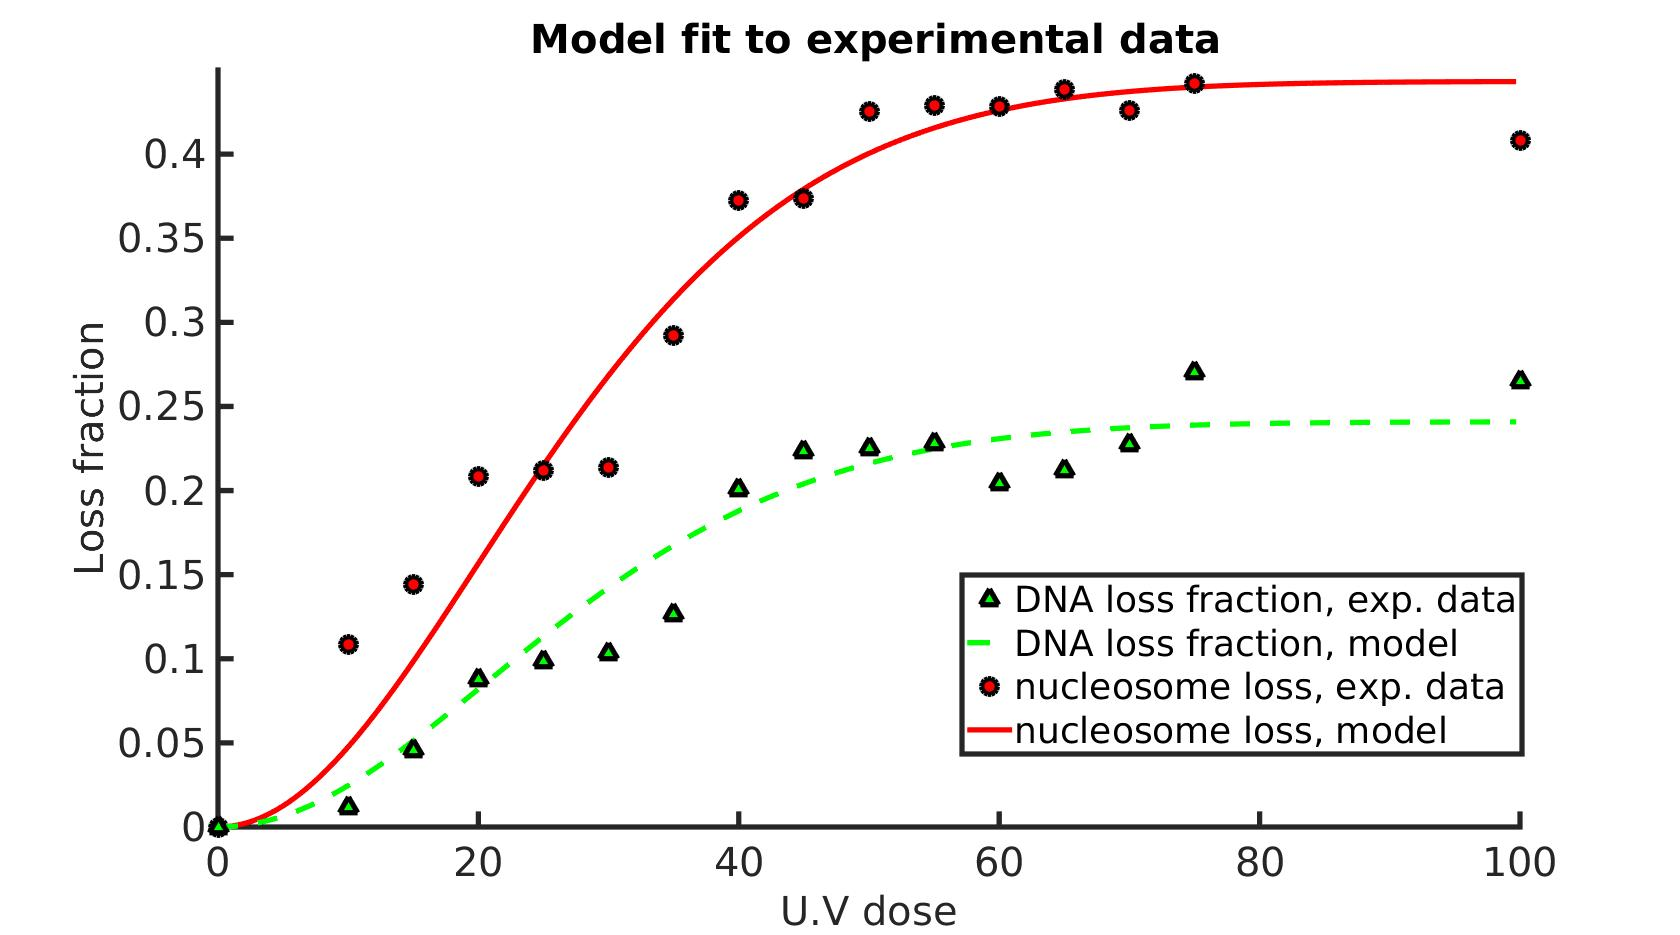
\includegraphics[width=0.5\linewidth, height=0.3\textheight]{histoneAndDnaVsUvDoseModelFit}
	\caption{\textbf{Histone (red) and DNA (green) loss: experimental data
		for nucleosomes (circle) and DNA (triangles) versus model curves
		(continuous and dashed, respectively)}. Parameter values are obtained
		by simultaneously fitting equations\eqref{eq:DNALoss}  and \eqref{eq:nucleosomeLoss} to the experimental data with
		the goal of maximizing the $R^2$. The resulting curves show $R^2 = 0.94$ and
		$R^2 = 0.955$ for DNA and nucleosome loss, respectively.}
	\label{fig:histoneAndDnaVsUvDoseModelFit}
	\end{figure}
	
   \subsection{Contribution of sliding and chromatin expansion to histone and DNA signal loss}
   equations \eqref{eq:relativeOpeningDNA}-\eqref{eq:relativeSlidingNucleosomes} are presented in Figure \ref{fig:relatiiveContributionToLoss}.
   		Using the calibrated models we have found that the relative contribution
   		of nucleosome sliding to the total signal loss in the ROI is monotonically
   		decreasing from 27.3\% to 24\% for DNA loss and from 62.5\% to 60\% for nucleosome signal,
   		as the UV dose increases from 0 to 100 msec. The remaining percentages are
   		attributed to chromatin expansion and de-compaction (see Figure \ref{fig:relatiiveContributionToLoss}).
   		
   		\begin{figure}[H]
   			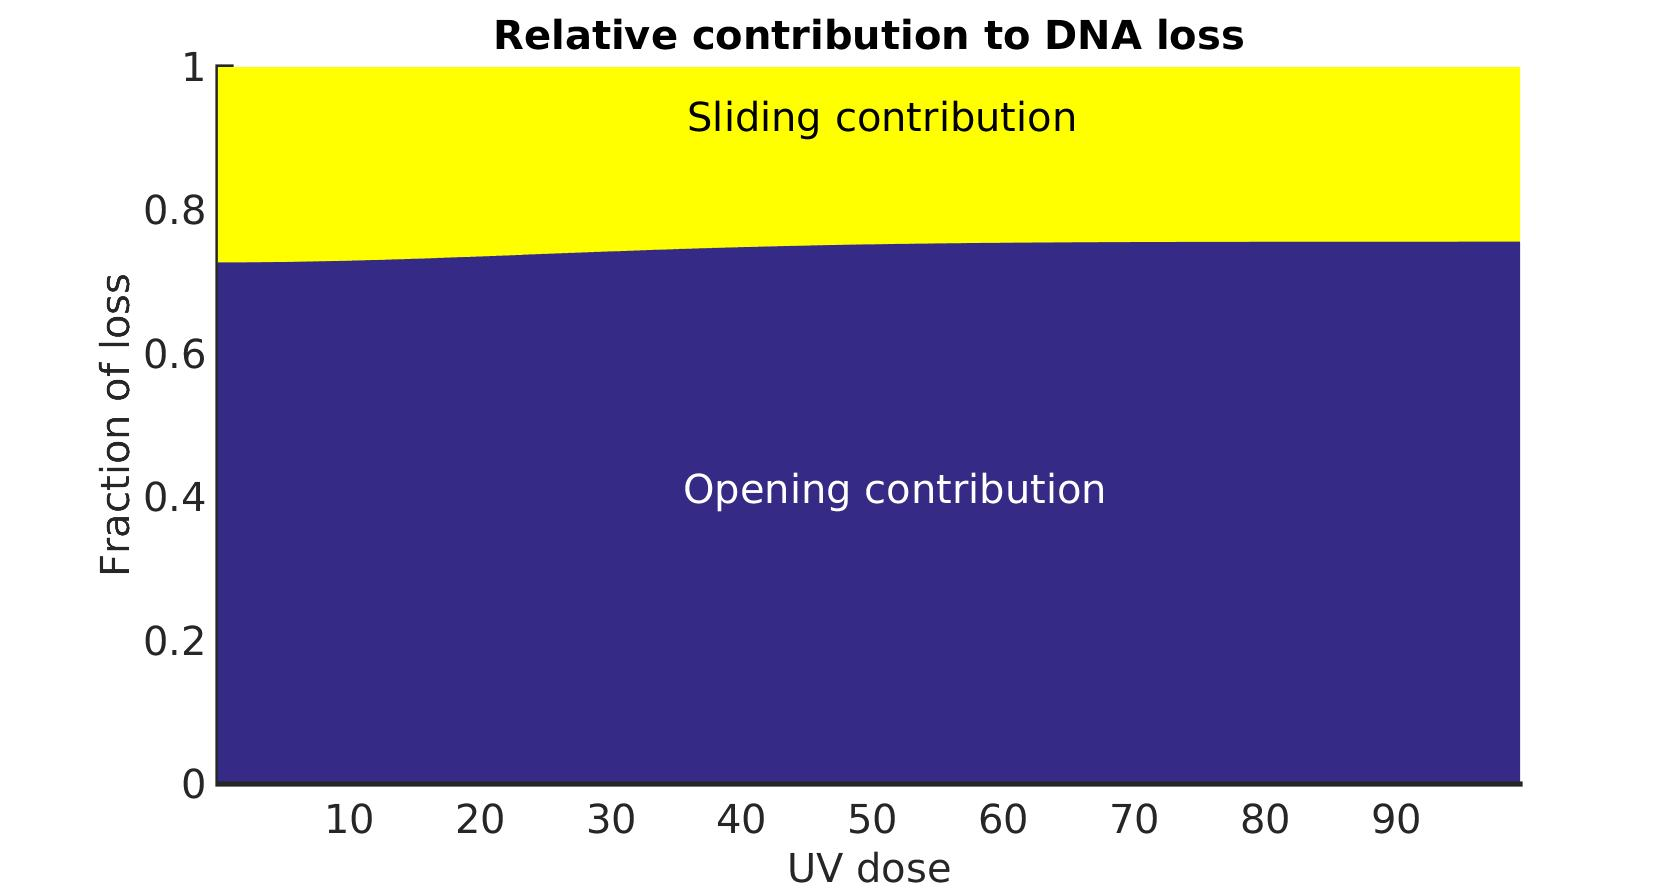
\includegraphics[width=0.5\linewidth, height=0.3\textheight]{relatiiveContributionToDNALoss}
   			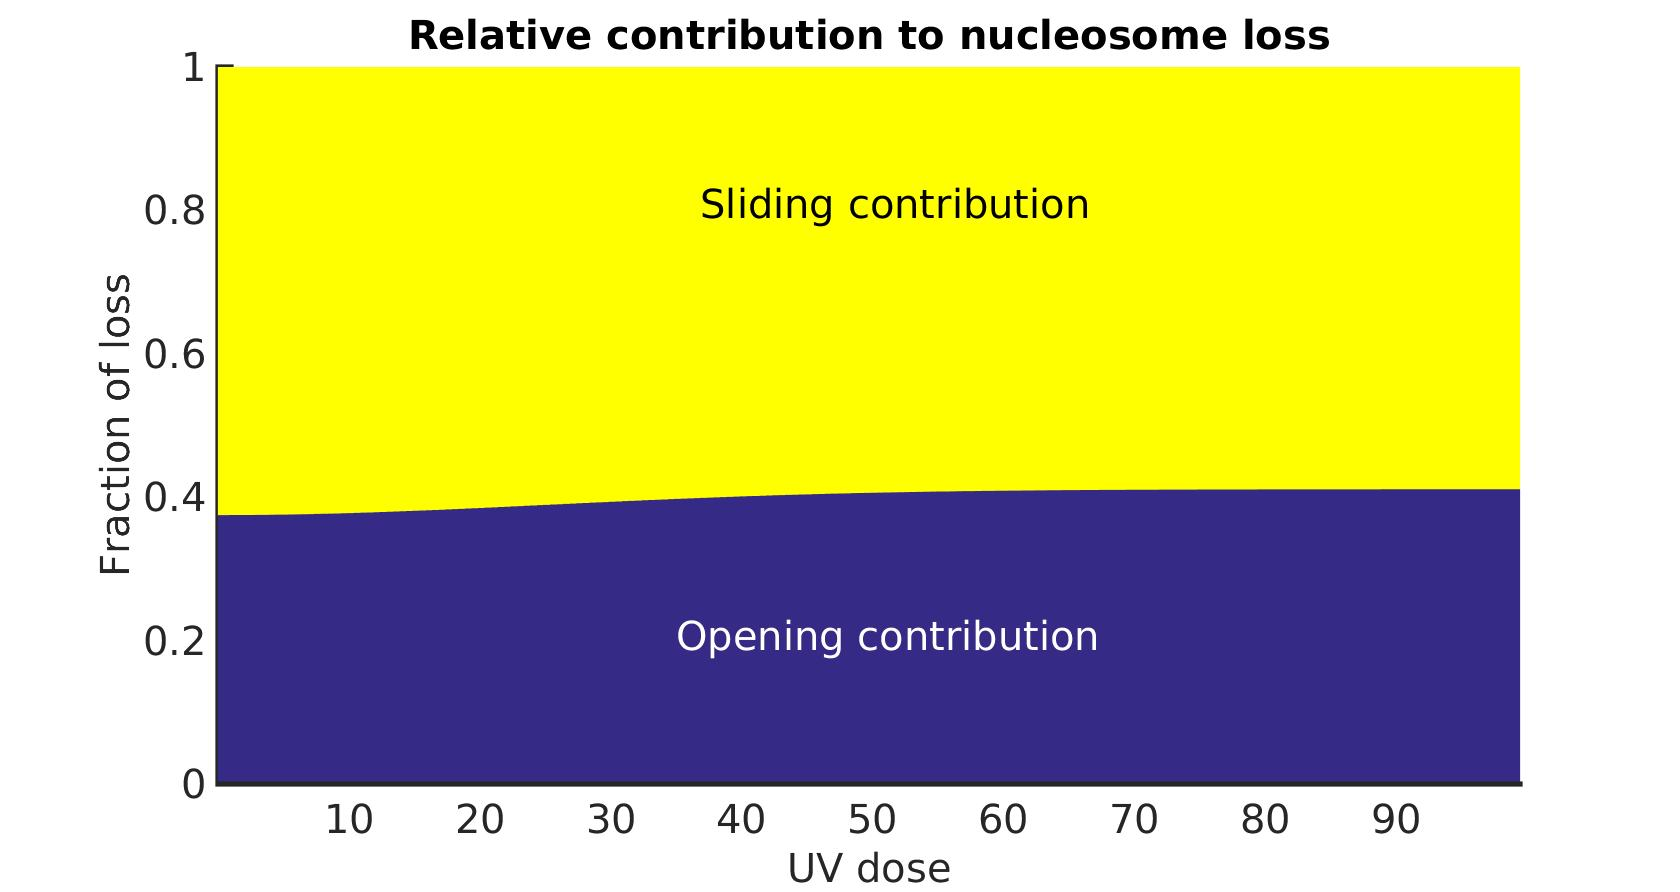
\includegraphics[width=0.5\linewidth, height=0.3\textheight]{relativeContributionToHistoneLoss}
   			\caption{\textbf{Relative contribution of chromatin opening and nucleosome sliding to DNA (left) and histone (right) loss}. Sliding contribution is monotonically decreasing with UV dose for both DNA and nucleosome signals.}
   			\label{fig:relatiiveContributionToLoss}
   		\end{figure}	
	\bibliographystyle{plain}
	\bibliography{ModelForHistoneSlidingChromatinStructurePostUVC} 
\end{document}